%%%%%%%%%%%%%%%%%%%%%%%%%%%%%%%%%%%%%%%%%%  不使用 authblk 包制作标题  %%%%%%%%%%%%%%%%%%%%%%%%%%%%%%%%%%%%%%%%%%%%%%
%-------------------------------PPT Title-------------------------------------
\title{07-\rm{PAW}方法简介}
%-----------------------------------------------------------------------------

%----------------------------Author & Date------------------------------------
%\author[\textrm{Jun\_Jiang}]{姜\;\;骏\inst{}} %[]{} (optional, use only with lots of authors)
%% - Give the names in the same order as the appear in the paper.
%% - Use the \inst{?} command only if the authors have different
%%   affiliation.
%\institute[BCC]{\inst{}%
\institute[Gain~Strong]{\inst{}%
%\vskip -20pt 北京市计算中心}
\vskip -20pt {\large 格致斯创~科技}}
\date[\today] % (optional, should be abbreviation of conference name)
{%	{\fontsize{6.2pt}{4.2pt}\selectfont{\textcolor{blue}{E-mail:~}\url{jiangjun@bcc.ac.cn}}}
\vskip 45 pt {\fontsize{8.2pt}{6.2pt}\selectfont{%清华大学\;\;物理系% 报告地点
	\vskip 5 pt \textrm{2023.02.24}}}
}

%% - Either use conference name or its abbreviation
%% - Not really information to the audience, more for people (including
%%   yourself) who are reading the slides onlin%%   yourself) who are reading the slides onlin%%   yourself) who are reading the slides onlineee
%%%%%%%%%%%%%%%%%%%%%%%%%%%%%%%%%%%%%%%%%%%%%%%%%%%%%%%%%%%%%%%%%%%%%%%%%%%%%%%%%%%%%%%%%%%%%%%%%%%%%%%%%%%%%%%%%%%%%

\subject{}
% This is only inserted into the PDF information catalog. Can be left
% out.
%\maketitle
\frame
{
%	\frametitle{\fontsize{9.5pt}{5.2pt}\selectfont{\textcolor{orange}{“高通量并发式材料计算算法与软件”年度检查}}}
\titlepage
}
%-----------------------------------------------------------------------------

%------------------------------------------------------------------------------列出全文 outline ---------------------------------------------------------------------------------
%\section*{}
%\frame[allowframebreaks]
%{
%  \frametitle{Outline}
%%  \frametitle{\textcolor{mycolor}{\secname}}
%  \tableofcontents%[current,currentsection,currentsubsection]
%}
%%在每个section之前列出全部Outline
%%类似的在每个subsection之前列出全部Outline是\AtBeginSubsection[]
%\AtBeginSection[]
%{
%  \frame<handout:0>%[allowframebreaks]
%  {
%    \frametitle{Outline}
%%全部Outline中,本部分加亮
%    \tableofcontents[current,currentsection]
%  }
%}

%-----------------------------------------------PPT main Body------------------------------------------------------------------------------------
\small
\section{\rm{PAW}方法}
\frame
{
	\frametitle{\textrm{PAW}方法概要}
\begin{itemize}
	\item 与芯层态正交的全部价电子构成的\textrm{Hilbert}空间%,价电子彼此的正交使得波函数在\textrm{Muffin-tin}球内振荡
	\item 作\textcolor{red}{线性空间变换},全电子波函数$|\Psi\rangle$与赝波函数$|\tilde\Psi\rangle$满足:
		$$|\Psi\rangle=\mathbf{\tau|}\tilde\Psi\rangle$$
%	$$\tau=\mathbf{1}+\sum_{\mathrm R}\hat\tau_{\mathrm R}$$
	\item 在原子核附近的$r_c$范围内,波函数用原子分波函数展开:
	$$|\Psi\rangle=|\tilde\Psi\rangle+\sum_i(|\phi_i\rangle-|\tilde\phi_i\rangle)\langle\tilde p_i|\tilde\Psi\rangle$$
	\item 在$r_c$外$|\tilde\Psi\rangle$与$|\Psi\rangle$变换前后保持不变,因此线性变换$\mathbf{\tau}$可表示为:
	$$\mathbf{\tau}=\mathbf{1}+\sum_i(|\phi_i\rangle-|\tilde\phi_i\rangle)\langle\tilde p_i|$$
\end{itemize}
其中$|\tilde p_i\rangle$是\textrm{MT}球内的投影函数\\
$i$表示原子位置$\vec R$、原子轨道($l,m$)和能级$\epsilon_k$的指标。
}

\frame
{
	\frametitle{\textrm{PAW}方法的基本思想}
	\vspace{10pt}
\begin{figure}[h!]
\centering
\includegraphics[height=1.8in,width=4.in,viewport=30 210 570 440,clip]{Figures/PAW_projector.eps}
\caption{\tiny \textrm{The analysis of PAW basic function.}}%(与文献\cite{EPJB33-47_2003}图1对比)
\label{PAW_baisc}
\end{figure}
}

\frame
{
\frametitle{\textrm{PAW}方法的基本思想}
	在赝波函数$|\tilde\Psi\rangle$表象下,算符期望值计算满足$$\langle A \rangle=\langle\Psi|\mathbf{A}|\Psi\rangle=\langle\tilde\Psi|\mathbf{\tau}^{\dag}\mathbf{A}\mathbf{\tau}|\tilde\Psi\rangle=\langle\tilde\Psi|\tilde{\mathrm{A}}|\tilde\Psi\rangle$$
\begin{itemize}
	\item 一般赝算符$\tilde A$表示为
		$$\tilde A=\mathbf{A}+\sum_i|\tilde p_i\rangle(\langle\phi_i|\mathbf{A}|\phi_i\rangle-\langle\tilde\phi_i|\mathbf{A}|\tilde\phi_i\rangle)\langle\tilde p_i|$$
	\item 赝重叠算符$\tilde O$表示为
		$$\tilde O=\mathbf{1}+\sum_i|\tilde p_i\rangle(\langle\phi_i|\phi_i\rangle-\langle\tilde\phi_i|\tilde\phi_i\rangle)\langle\tilde p_i|$$
\end{itemize}
}

\frame
{
\frametitle{\textrm{PAW}方法密度计算}
在\textrm{PAW}框架下,将密度算符$|\vec r\rangle\langle\vec r|$代入,可知密度表达式为
$$n(\vec r)=\tilde n(\vec r)+n^1(\vec r)-\tilde n^1(\vec r)$$
这里
$$\tilde n(\vec r)=\sum_nf_n\langle\tilde\Psi_n|\vec r\rangle\langle\vec r|\tilde\Psi_n\rangle$$ 
$$n^1(\vec r)=\sum_{n,(i,j)}f_n\langle\tilde\Psi_n|\tilde p_i\rangle\langle\phi_i|\vec r\rangle\langle\vec r|\phi_j\rangle\langle\tilde p_j|\tilde\Psi_n\rangle$$
$$\tilde n^1(\vec r)=\sum_{n,(i,j)}f_n\langle\tilde\Psi_n|\tilde p_i\rangle\langle\tilde\phi_i|\vec r\rangle\langle\vec r|\tilde\phi_j\rangle\langle\tilde p_j|\tilde\Psi_n\rangle$$
}

\frame
{
\frametitle{\textrm{PAW}方法总能量的计算}
总能量泛函
%\begin{displaymath}
%	\begin{aligned}
%		E&=\sum_nf_n\langle\Psi_n|-\dfrac12\nabla^2|\Psi_n\rangle\\
%		 &+\dfrac12\int\mathrm{d}\vec r\int\mathrm{d}\vec r^{\prime}\dfrac{(n+n^Z)(n+n^Z)}{|\vec r-\vec r^{\prime}|}+\int\mathrm{d}\vec r n\epsilon_{\mathrm{XC}}(n)
%	\end{aligned}
%\end{displaymath}
$E=\tilde E+E^1-\tilde E^1$,每一项分别表示为:
\begin{displaymath}
	\begin{aligned}
		\tilde E&=\sum_nf_n\langle\tilde\Psi_n|-\dfrac12\nabla^2|\tilde\Psi_n\rangle\\
		 &+\dfrac12\int\mathrm{d}\vec r\int\mathrm{d}\vec r^{\prime}\dfrac{(\tilde n+\hat n)(\tilde n+\hat n)}{|\vec r-\vec r^{\prime}|}+\int\mathrm{d}\vec r \tilde n\bar v+\int\mathrm{d}\vec r \tilde n\epsilon_{\mathrm{XC}}(\tilde n)
 	\end{aligned}
\end{displaymath}
\begin{displaymath}
	\begin{aligned}
		E^1&=\sum_{n,(i,j)}f_n\langle\tilde\Psi_n|\tilde p_i\rangle\langle\phi_i|-\dfrac12\nabla^2|\phi_j\rangle\langle\tilde p_j|\tilde\Psi_n\rangle\\
		 &+\dfrac12\int\mathrm{d}\vec r\int\mathrm{d}\vec r^{\prime}\dfrac{(n^1+n^Z)(n^1+n^Z)}{|\vec r-\vec r^{\prime}|}+\int\mathrm{d}\vec r n^1\epsilon_{\mathrm{XC}}(n^1)
 	\end{aligned}
\end{displaymath}
\begin{displaymath}
	\begin{aligned}
		\tilde E^1&=\sum_{n,(i,j)}f_n\langle\tilde\Psi_n|\tilde p_i\rangle\langle\tilde\phi_i|-\dfrac12\nabla^2|\tilde\phi_j\rangle\langle\tilde p_j|\tilde\Psi_n\rangle\\
		 &+\dfrac12\int\mathrm{d}\vec r\int\mathrm{d}\vec r^{\prime}\dfrac{(\tilde n^1+\hat n)(\tilde n^1+\hat n)}{|\vec r-\vec r^{\prime}|}+\int\mathrm{d}\vec r \tilde n^1\bar v+\int\mathrm{d}\vec r \tilde n^1\epsilon_{\mathrm{XC}}(\tilde n^1)
 	\end{aligned}
\end{displaymath}
}

%\subsection{\rm{PAW}的实现}
\frame
{
	\frametitle{补偿电荷的表示}
	补偿电荷$\hat n$要求局域在缀加区(\textrm{Augmentation region}),可表示为
	$$\hat n=\sum_R\hat n_R$$
	其中$\hat n_R$是单个原子截断区间的补偿电荷,可以表示为广义的\textrm{Gaussian}函数的求和
	$$\hat n_R(r)=\sum_{L=(l,m)}g_{RL}(r)Q_{RL}$$
	其中$g_{RL}(r)$表示为
	$$g_{RL}(r)=C_l|r-R|^lY_L(r-R)\mathrm{e}^{-(|r-R|/r_c)^2}$$
	系数$C_l$是归一化系数,由条件
	$\int\mathrm{d}rr^lY_L(r)g_L(r)=1$
	确定

	$Q_{RL}$是补偿电荷要满足的多极矩
	$$Q_{RL}=\int\mathrm{d}r|r-R|^l\big[n_R^1(r)+n_R^Z(r)-\tilde n_R^1(r)\big]Y_L^{\ast}(r-R)$$
}

\frame
{
\frametitle{补偿电荷与多极矩}
根据电动力学定理:\\\textcolor{blue}{如果球\textrm{S}内的电荷密度分布$\rho(\vec r)$,在球外某点$\vec r$产生的势是由电荷密度的多极矩确定}:
\begin{figure}[h!]
\vspace*{-15pt}
\centering
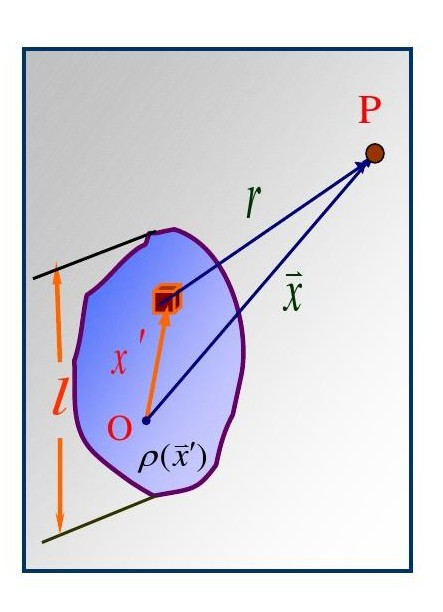
\includegraphics[height=1.25in,width=1.32in,viewport=1 22 507 575,clip]{Figures/potential_multipole.jpg}
%\caption{\tiny \textrm{From Muffin-tin Potential to Full Potential}}%(与文献\cite{EPJB33-47_2003}图1对比)
\label{Potential-multipole}
\end{figure}
\begin{displaymath}
	V(\vec r)=\sum_{l=0}^{\infty}\sum_{m=-l}^{l}\dfrac{4\pi}{2l+1}q_{lm}\dfrac{Y_{lm}(\hat{\vec r})}{r^{l+1}}
\end{displaymath}
其中多极矩$q_{lm}$由下式计算
\begin{displaymath}
	q_{lm}=\int_SY_{lm}^{\ast}(\hat{\vec r})r^l\rho(\vec r)\mathrm{d}^3r
\end{displaymath}
}

\frame
{
	\frametitle{补偿电荷与能量$\tilde E$}
	如果要求\textrm{Gaussian}函数在缀加区衰减,则需要用很高的\textrm{Fourier}截断,这意味着需要很高的平面波能量截断。引入补偿电荷$\hat n^{\prime}$,要求满足条件
	\begin{itemize}
		\item $\hat n^{\prime}$与$\hat n$具有相同的多极矩
		\item $\hat n^{\prime}$对应的\textrm{Gaussian}函数的衰减半径$r_c^{\prime}$比$r_c$大得多,可以用很少的平面波展开
	\end{itemize}
	因此能量$\tilde E$中的\textcolor{blue}{静电相互作用}可以表示为
	\begin{displaymath}
		\begin{aligned}
			&\dfrac12\int\mathrm{d}r\int\mathrm{d}r^{\prime}\dfrac{(\tilde n+\hat n)(\tilde n+\hat n)}{|r-r^{\prime}|}\\
			=&\underline{\dfrac12\int\mathrm{d}r\int\mathrm{d}r^{\prime}\dfrac{(\tilde n+\hat n^{\prime})(\tilde n+\hat n^{\prime})}{|r-r^{\prime}|}}
			+\underline{\int\mathrm{d}r\tilde n(r)\hat v(r)}+\underline{\sum_{R,R^{\prime}}U_{R,R^{\prime}}}
		\end{aligned}
	\end{displaymath}
}

\frame
{
	\frametitle{能量$\tilde E$的静电相互作用分解}
	其中第一项是平滑函数,可以在\textrm{Fourier}空间计算
	$$2\pi V\sum_G\dfrac{|\tilde n(G)+\hat n^{\prime}(G)|^2}{G^2}$$
	第二项的$\hat v(r)$表示为
	$$\hat v(r)=\int\mathrm{d}r^{\prime}\dfrac{\hat n(r^{\prime})-\hat n^{\prime}(r^{\prime})}{|r-r^{\prime}|}$$
	虽然$\hat v(r)$和$n(r)$一样有高\textrm{Fourier}截断,但\textcolor{red}{高阶部分不会对$\int\mathrm{d}r\tilde n(r)\hat v(r)$有贡献}

	最后一项中$U_{R,R^{\prime}}$是原子间的短程成对势
	$$U_{R,R^{\prime}}=\dfrac12\int\mathrm{d}r\int\mathrm{d}r^{\prime}\dfrac{\hat n_R(r)\hat n_{R^{\prime}}(r^{\prime})-\hat n_R^{\prime}(r)\hat n_{R^{\prime}}^{\prime}(r^{\prime})}{|r-r^{\prime}|}$$
	这一项\textcolor{blue}{可以通过\textrm{Ewald}求和方法计算}
}

\frame
{
	\frametitle{重叠矩阵和\textrm{Hamiltonian}矩阵}
重叠算符:
$$\tilde O=1+\sum_{i,j}|\tilde p_i\rangle\bigg[\langle\phi_i|\phi_j\rangle-\langle\tilde\phi_i|\tilde\phi_j\rangle\bigg]\langle\tilde p_j|$$
\textrm{Hamilitonian}算符:
%\begin{itemize}
%	\item 动能算符:
%		$$\tilde T=-\dfrac12\nabla^2+\sum_{i,j}|\tilde p_i\rangle[\langle\phi_i|-\dfrac12\nabla^2|\phi_j\rangle-\langle\tilde\phi_i|-\dfrac12\nabla^2|\tilde\phi_j\rangle]\langle\tilde p_j|$$
%	\item 完全势\textrm{(full-potential)}算符:
%$$v(\vec r)=\tilde v(\vec r)+v^1(\vec r)-\tilde v^1(\vec r)$$
%	\item \textrm{Hamilton}算符:
\begin{displaymath}
	\begin{aligned}
		\tilde H=&-\dfrac12\nabla^2+\tilde v+\sum_{i,j}|\tilde p_i\rangle\bigg[\langle\phi_i|-\dfrac12\nabla^2+v^1|\phi_j\rangle\\
			&-\langle\tilde\phi_i|-\dfrac12\nabla^2+\tilde v^1|\tilde\phi_j\rangle\bigg]\langle\tilde p_j| 
	\end{aligned}
\end{displaymath}
%\end{itemize}
	完整的势函数\textrm{(full-potential)}算符:
$$v(\vec r)=\tilde v(\vec r)+v^1(\vec r)-\tilde v^1(\vec r)$$
因此可以有
$$\left.\dfrac{\partial E[\tilde\Psi, R]}{\partial\langle\tilde\Psi_n|}\right|_R=\tilde H|\tilde\Psi_n\rangle f_n$$
}

\frame
{
	\frametitle{\textrm{PAW}原子数据集}
\textrm{PAW}原子数据集是在原子核附近$r_c$范围内将波函数用原子分波展开所需信息的统称,是\textrm{PAW}计算的基础。

\textrm{PAW}原子数据集主要包括
	\begin{itemize}
		\item 分波信息:原子分波$\phi_i$、赝分波$\tilde\phi_i$和投影子波函数$\tilde{p}_i$
		\item 密度信息:$r_c$内的电荷密度$n^1$、赝电荷密度$\tilde n^1$和补充电荷$\hat n$
		\item 赝势信息:局域赝势$\tilde v_{loc}(\vec r)$
	\end{itemize}
	与赝势方法相似,一套原子数据集将用于各种化学环境下的\textrm{PAW}计算,即要求原子数据集有良好的可移植性;与赝势方法不同之处在于\textrm{PAW}原子集中除了赝原子的信息,还包含了真实原子的信息。
}

\frame
{
	\frametitle{\textrm{PAW}原子数据集:~实现方案}
	\fontsize{7.2pt}{5.2pt}\selectfont{原子分波:$$\bigg(-\dfrac12\nabla^2+v_{at}-\varepsilon_i^1\bigg)|\phi_i\rangle=0$$
	赝原子分波:$$\bigg(-\dfrac12\nabla^2+w_i(r)-\varepsilon_i^1\bigg)|\tilde\phi_i\rangle=0$$
	局域赝势:% $$w_i(r)=\tilde v_{at}(r)+c_ik(r)=\tilde v_{at}(0)\mathrm{e}^{-(r/r_k)^{\lambda}}+[1-k(r)]v_{at}(r)+c_i\mathrm{e}^{-(r/r_k)^{\lambda}}$$
	\begin{itemize}
		\item 过渡金属体系:~采用带参数的四阶多项式,要求赝波函数在截断半径处保持与真实波函数相同的连续可微
		\item 价层不含$d$电子电子体系:引入截断函数
			\begin{displaymath}
				k(r)=\exp[-(r/r_k)^{\lambda}]
			\end{displaymath}
			定义有效(局域)赝势
			\begin{displaymath}
				\textcolor{red}{\tilde v_{\mathrm{at}}(r)} = \tilde v_{\mathrm{at}}(0)k(r)+[1-k(r)]v_{\mathrm{at}}(r)
			\end{displaymath}
			调节截断半径$r_k$和指数$\lambda$,使得赝原子势和真实原子势在截断半径外严格相等
	\end{itemize}
	\vskip 5pt
	实际求解赝波函数时的赝势定义为
\begin{displaymath}
	w_i(r)=\textcolor{red}{\tilde v_{\mathrm{at}}(r)}+\textcolor{blue}{\boxed{c_ik(r)}~\Leftarrow~{\mathrm{non~local~part~of~the~pseudo potential}}}
\end{displaymath}
调节参数$c_i$使得要求赝波函数与真实波函数在截断截断半径外完全相同
%	$$w_i(r)=\tilde v_{at}(0)\mathrm{e}^{-(r/r_k)^{\lambda}}+[1-\mathrm{e}^{-(r/r_k)^{\lambda}}]v_{at}(r)+c_i\mathrm{e}^{-(r/r_k)^{\lambda}}$$
}
}

\frame
{
	\frametitle{\textrm{可移植离子局域势$\bar v$}}
	%对于\textcolor{red}{束缚态},
	\fontsize{9.2pt}{7.2pt}\selectfont{参照局域赝势去屏蔽方案,扣除赝势中的赝分波部分的贡献,将得到可移植性更好的离子局域势:
	$$\bar v(r)=\tilde v_{at}(r)-\int\mathrm{d}r^{\prime}\dfrac{\tilde n(r^{\prime})+\hat n(r^{\prime})}{|r-r^{\prime}|}-\mu_{xc}[\tilde n(r)]$$
	\textcolor{magenta}{赝分波$\tilde\phi_j$并不一定对应原子束缚态},但要满足以下广义本征值方程
	$$\bigg[-\dfrac12\nabla^2+\tilde v_{at}-\varepsilon+\sum_{(i,j)}|\tilde p_i\rangle\big(\mathrm{d}H_{ij}-\varepsilon\mathrm{d}O_{ij}\big)\langle\tilde p_j|\bigg]|\tilde\phi_j\rangle=0$$
	其中$\mathrm{d}H_{ij}$和$\mathrm{d}O_{ij}$分别是
	$$\mathrm{d}H_{ij}=\langle\phi_i|-\dfrac12\nabla^2+v_{at}|\phi_j\rangle-\langle\tilde\phi_i|-\dfrac12\nabla^2+\tilde v_{at}|\tilde\phi_j\rangle$$
	$$\mathrm{d}O_{ij}=\langle\phi_i|\phi_j\rangle-\langle\tilde\phi_i|\tilde\phi_j\rangle$$}
}

\frame
{
	\frametitle{赝分波函数的求解}
	为检验赝势的散射性质,还要考虑赝势的可分离特征:\\
	上述广义本征值方程是非齐次的,可假设其解形式为
	$$|\tilde\phi\rangle=|u\rangle+\sum_i|w_i\rangle c_i$$
	其中$|u\rangle$和$|w_i\rangle$的定义分别为
	$$\big(-\frac12\nabla^2+\tilde v_{\mathrm{at}}-\varepsilon\big)|u\rangle=0$$
	$$\big(-\frac12\nabla^2+\tilde v_{\mathrm{at}}-\varepsilon\big)|w_i\rangle=|\tilde p_i\rangle$$
	由此可得到
	$$c_i=-\sum_{j,l}\bigg[\delta_{ij}+\sum_k\mathrm{d}H_{ik}-\varepsilon\mathrm{d}O_{ik}\langle\tilde p_k|w_j\rangle\bigg]^{-1}\big(\mathrm{d}H_{jl}-\varepsilon\mathrm{d}O_{jl}\big)\langle\tilde p_l|u\rangle$$
}

\frame
{
	\frametitle{\textrm{PAW projector}:~实现方案}
	\textcolor{red}{预设投影函数}:$$\textcolor{red}{|\tilde p_i\rangle}=\bigg(-\dfrac12\nabla^2+\tilde v_{at}-\varepsilon_i^1\bigg)|\tilde\phi_i\rangle$$
	\textcolor{blue}{当预设投影函数为0时}(对应局域势),\textcolor{blue}{投影函数即为截断函数$k(r)$}
\begin{minipage}[t]{0.52\linewidth}
\begin{figure}[h!]
\centering
\vspace*{-0.30in}
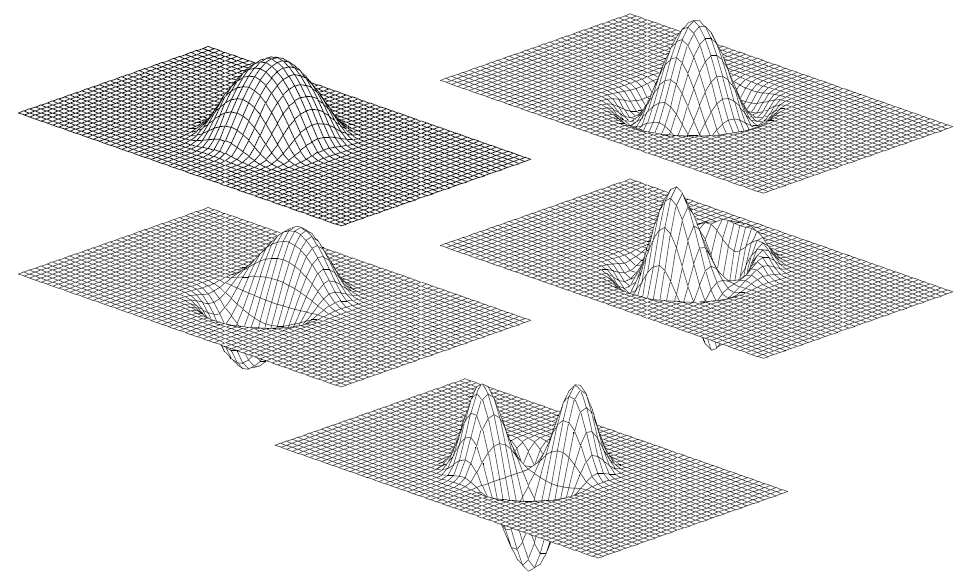
\includegraphics[height=1.2in,width=1.8in,viewport=0 0 1100 745,clip]{Figures/PAW_projector-2.png}
\caption{\tiny \textrm{The projector of PAW.}}%(与文献\cite{EPJB33-47_2003}图1对比)
\label{PAW_projector}
\end{figure}
\end{minipage}
\hfill
\begin{minipage}[t]{0.43\linewidth}
\begin{itemize}
	\item 与分波具有相同的$l$值
	\item 局域在缀加区域(\textrm{Augmentation region})
	\item 节点依次增加
\end{itemize}
\end{minipage}
	\fontsize{7.2pt}{5.2pt}\selectfont{\textrm{Gram-Schmidt}正交化
	$$|\tilde p_i\rangle=|\tilde p_i\rangle-\sum_{j=1}^{i-1}|\tilde p_j\rangle\langle\tilde\phi_j|\tilde p_i\rangle$$
%	$$|\phi_i\rangle=|\phi_i\rangle-\sum_{j=1}^{i-1}|\phi_j\rangle\langle\tilde p_j|\tilde\phi_i\rangle$$
%	$$|\tilde\phi_i\rangle=|\tilde\phi_i\rangle-\sum_{j=1}^{i-1}|\tilde\phi_j\rangle\langle\tilde p_j|\tilde\phi_i\rangle$$
	$$|\phi_i\rangle=|\phi_i\rangle-\sum\limits_{j=1}^{i-1}|\phi_j\rangle\langle\tilde p_j|\tilde\phi_i\rangle\quad|\tilde\phi_i\rangle=|\tilde\phi_i\rangle-\sum\limits_{j=1}^{i-1}|\tilde\phi_j\rangle\langle\tilde p_j|\tilde\phi_i\rangle$$}
}

\frame
{
	\frametitle{\textrm{PAW}原子数据集:~示例}
\begin{figure}[h!]
\centering
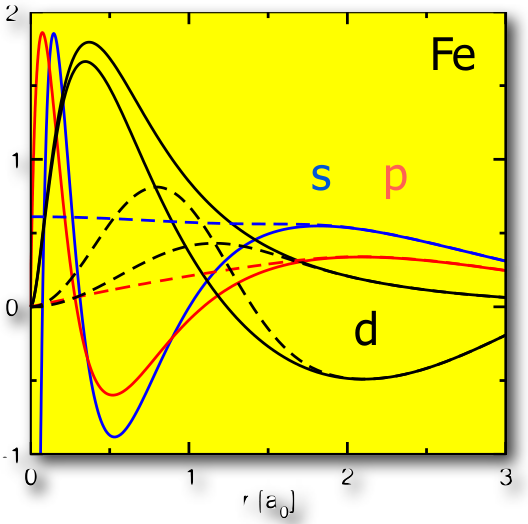
\includegraphics[height=2.5in,width=3.3in,viewport=0 0 570 545,clip]{Figures/PAW-partical.png}
\caption{\tiny \textrm{The partical-wave of Fe atom.}}%(与文献\cite{EPJB33-47_2003}图1对比)
\label{PAW_partical_Fe}
\end{figure}
}

\frame
{
	\frametitle{几种赝势方法的关系}
\begin{figure}[h!]
\centering
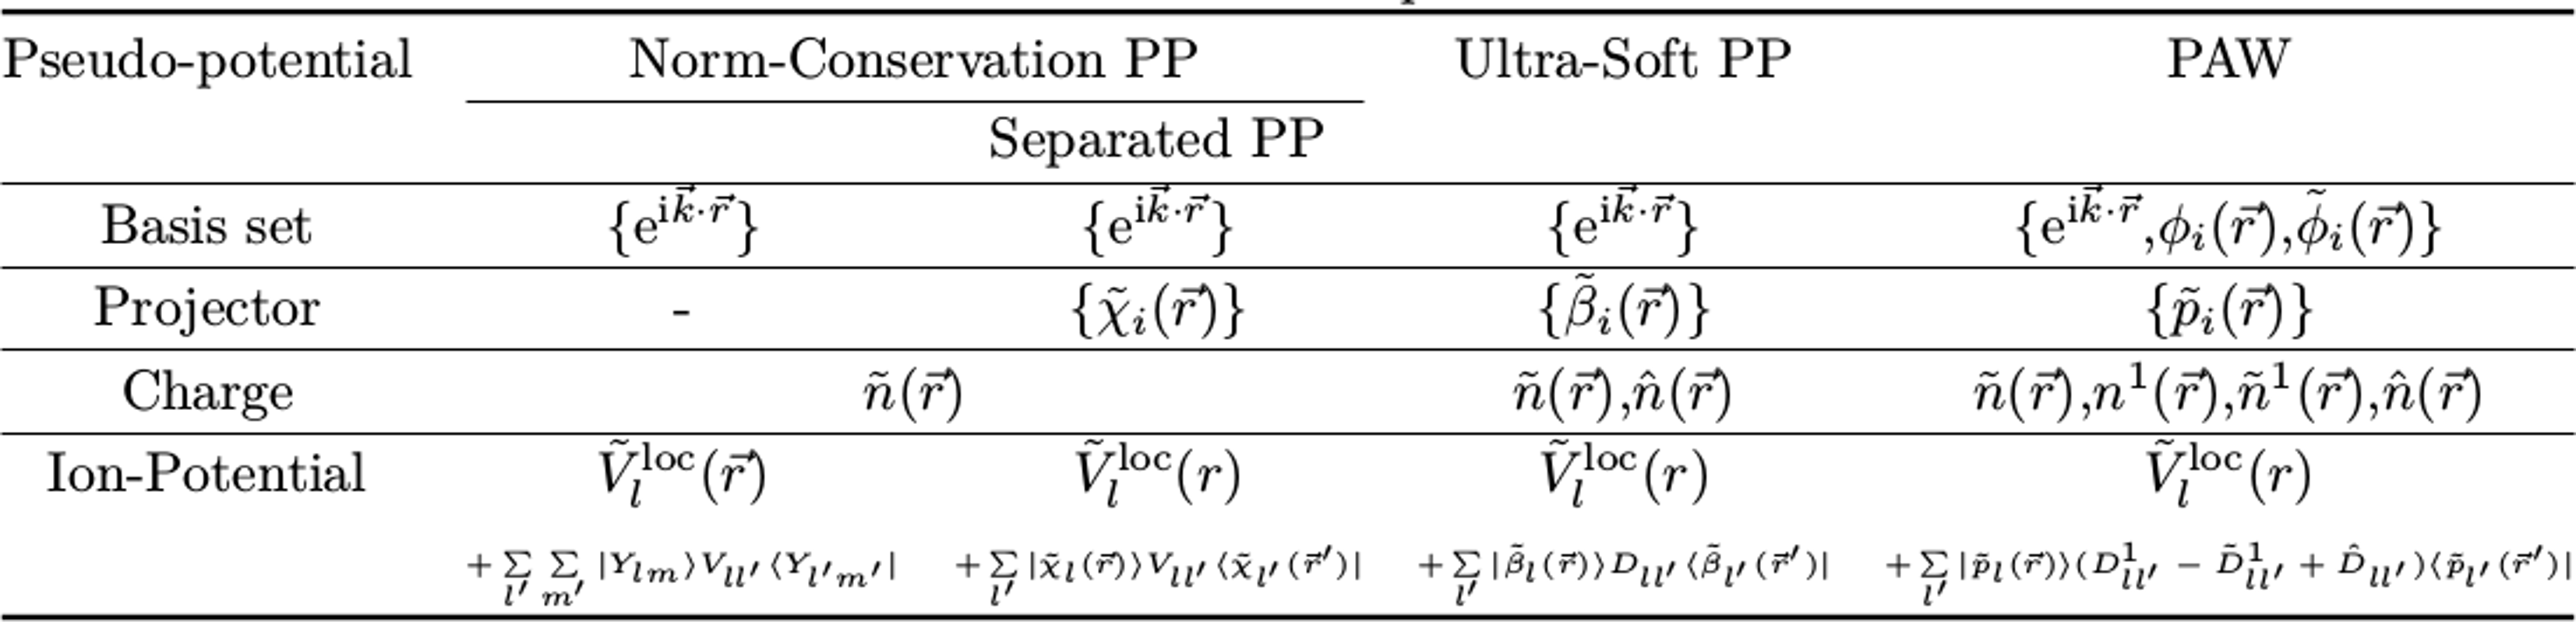
\includegraphics[height=1.0in,width=4.1in,clip]{Figures/Pseudo-Potential.png}
\caption{\tiny \textrm{The relation of Pseudo potential and PAW.}}%(与文献\cite{EPJB33-47_2003}图1对比)
\label{Pseudo_Potential_PAW}
\end{figure}
}
